\documentclass[11pt]{article}

% Packages and macros go here
\usepackage{graphicx}
\usepackage{tabu}
\usepackage{subcaption}
\usepackage{lipsum}
\usepackage{amsfonts}
\usepackage{epstopdf}
\usepackage[lined,boxed]{algorithm2e}
\usepackage{booktabs}
\usepackage{subcaption}
\usepackage{esvect}
\usepackage{tikz}
\definecolor{vertB}{RGB}{20, 148, 20}
\usepackage{multirow}
\usepackage{amsmath}
\usepackage{amssymb}
\usepackage{caption}

\usepackage{changes}
\usepackage{todonotes}% See
% http://tug.ctan.org/macros/latex/contrib/changes/changes.english.pdf for documentation
\definechangesauthor[name={Luiz Faria},color=blue]{lmf}
% \newcommand{\missing}[1]{\todo[color=red]{#1}}
\newcommand{\improvement}[1]{\todo[color=orange]{#1}}
\newcommand{\question}[1]{\todo[color=yellow]{#1}}

\usepackage{multirow}
\usepackage{amsmath}
\usepackage{amsfonts}
\usepackage{amsmath}
\usepackage{amssymb}
\usepackage{graphicx}
\usepackage{caption}
\usepackage{enumitem}
\usepackage{mathrsfs}
\usepackage{upgreek}
\usepackage{amsthm}
\usepackage{booktabs}
\usepackage{authblk}
\usepackage[noabbrev]{cleveref}
\crefformat{equation}{(#2#1#3)}

\newcommand{\pder}[2]{\frac{\partial #1}{\partial #2}}
\newcommand{\R}{\mathbb{R}}
\newcommand{\C}{\mathbb{C}}
\newcommand{\N}{\mathbb{N}}
\newcommand{\bn}{\mathbf{n}}
\newcommand{\bx}{\mathbf{x}}
\newcommand{\bz}{\mathbf{z}}
\newcommand{\btau}{\boldsymbol{\tau}}
\newcommand{\bhx}{{\mathbf{\hat{x}}}}
\newcommand{\bhy}{\mathbf{\hat{y}}}
\newcommand{\hx}{{\hat{x}}}
\newcommand{\hy}{{\hat{y}}}
\newcommand{\hvarphi}{{\hat{\varphi}}}
\newcommand{\hPhi}{{\hat{\Phi}}}
\newcommand{\by}{\mathbf{y}}
\newcommand{\br}{\boldsymbol{r}}
\newcommand{\btheta}{\mathbf{\theta}}
\newcommand{\de}{\,\mathrm{d}}
\newcommand{\htau}{{\hat{\tau}}}
\newcommand{\hpsi}{{\hat{\psi}}}
\newcommand{\M}{\mathcal{T}}
\newcommand{\surface}{\Gamma_{f}}
\newcommand{\solid}{\Gamma_{s}}
\newcommand{\tvarphi}{\tilde \varphi}

%%%%%%%%%%%%%%%%%%%%%%
\newtheorem{theorem}{Theorem}[section]
\newtheorem{lemma}[theorem]{Lemma}
\newtheorem{proposition}[theorem]{Proposition}
\newtheorem{corollary}[theorem]{Corollary}
\newtheorem{remark}[theorem]{Remark}
\newtheorem{definition}[theorem]{Definition}

\topmargin -.5in
\oddsidemargin 0pt
\textheight 8.8in
\textwidth 6.5in

\title{Complex-scaled boundary integral equation for time-harmonic water waves}

\author[1]{Anne-Sophie Bonnet-Bendhia \thanks{anne-sophie.bonnet-bendhia@ensta-paristech.fr}}
\author[1]{Luiz M. Faria\thanks{luiz.maltez-faria@inria.fr}}
\author[2]{Carlos Perez-Arancibia\thanks{c.a.perezarancibia@utwente.nl}}
\affil[1]{\small{Laboratoire POEMS, CNRS/ENSTA/INRIA, France}}
\affil[2]{\small{Univeristy of Twente, Netherlands}}

\date{\today}

\begin{document}

\maketitle

% REQUIRED
\begin{abstract}  
  We present a novel boundary integral equation (BIE) formulation for
  time-harmonic water-waves problem based on the complexification of Laplace's
  free-space Green function. The method employs a perfectly matched layer (PML)
  coordinate-stretching to render the propagative waves exponentially decaying,
  thus facilitating the truncation of the unbounded interfaces comprised by the
  free-surface and the bottom topography. The formulation uses only simple
  function evaluations (e.g. complex logarithms and square roots), avoiding the
  use of the water-wave Green’s function. We show through a variety of numerical
  examples that the truncation errors are exponentially small with respect to a
  parameter $\ell$ controlling the length of the PML layer.
\end{abstract}

% REQUIRED
 \textbf{Keywords}: Perfectly matched layers, boundary integral equations \\

%\noindent \textbf{AMS subject classifications}:

\tableofcontents

\section{Introduction}

Solving partial differential equations (PDEs) on unbounded domains poses
additional challenges from both a theoretical and numerical point of view.
Theoretically, one is required to impose appropriate conditions at infinity to
guarantee uniqueness of solutions; when the underlying PDE comes from the
modeling of the physical world, additional care must be taken to also ensure the
recovered (unique) solution is the ``physically relevant'' one. The numerical
challenges, on the other hand, stem from the fact that the discretization scheme
should incorporate information about the boundary conditions at infinity, also
called radiation condition; this can be done directly, by e.g. expanding the
solution in a basis which satisfy the radiation condition, or indirectly by
truncating the domain to a finite size and imposing instead a carefully chosen
boundary condition on the artificial boundaries of the truncated domain.

In the case of volume discretization methods such as finite difference and
finite elements, a particular class of truncation techniques which enjoys great
popularity due to its accuracy and simplicity is the Perfectly Matched Layers
(PMLs) method. Loosely speaking, the method consists of solving for the analytic
extension of the sought solution which decays exponentially at infinity. The
decay rate of the analytic extension then facilitates the truncation of the
domain upon discretization. On the physical (i.e. real) domain, PMLs can be
reinterpreted as surrounding the computational region by a material layer, not
necessarily physical, which absorbs but does not reflect incoming waves. A key
difference between PMLs and \emph{ad hoc} absorbing material methods stem from
the fact that the PML absorbing material is ``perfect'' in the sense that it is
reflectionless at the continuous level (i.e. before discretization).

An alternative to volume discretization methods are boundary integral equation
methods, which rely on the use of a Green function to recast the PDE in terms of
integral operators over the interfaces where the medium changes property. For
piece-wise homogeneous media, this reduces the PDE to integral equations posed
at the interface between the different media. Because boundary integral methods
represent the solution as a sum of fundamental solutions which satisfy the
radiation boundary condition, no domain truncation technique is required when
the interfaces are bounded. This is a well-known advantage of boundary integral
methods for scattering problems. There are interesting cases, however, where
such interfaces are better modeled as infinite. Examples include the scattering
of an object near the ground, the propagation of elastic waves under the surface
of the earth, wave-guides, and the water-waves problem described below. In such
cases a truncation technique is required, at least in the direction parallel to
the infinite interfaces, to reduce the problem to a finite subdomain where the
equations can be discretized.

In order to handle infinite interfaces in a boundary integral equation context,
a few options are available. For relatively simple geometries and boundary
conditions, one can construct a problem specific Greens function which
incorporates the boundary condition on all but a bounded portion of the
interface, thus reducing the problem again to integrals over bounded
curves/surfaces. This has the advantage of being conceptually simple provided
such problem-specific Greens function can be efficiently computed.
Unfortunately, for all but the simplest geometries, the representation of the
problem specific Greens function involves challenging integrals which must be
approximated numerically. Alternatives which rely instead on the use of the
free-space Greens function, readily available for many PDEs of physical
relevance, have also been developed. In \cite{perez2017windowed} a high-order
method called the Windowed-Green function (WGF) was introduced in order to
truncate the integrals stemming from the boundary integral representation of the
unbounded interfaces in the context of two- and three-dimensional
Helmholtz/Maxwell scattering problems. At a similar time, \cite{lu2018perfectly}
proposed a technique based on combining perfectly matched layers and a boundary
integral representation on a certain truncated domain in the context of
two-dimensional Helmholtz scattering problems. 
% Due to the exponential decay of the Helmholtz Green function on the
% complex-scaled PML layer, the kernels of the integral operators over the
% infinite interfaces become exponentially small, allowing for an efficient
% truncation with errors that decay exponentially respect to a truncation
% parameter $\ell$ controlling the PML length. 
It is worth mentioning the naive approach of simply truncating the domain far
enough from the region of interest is rather unsatisfactory, specially for
non-dissipative PDEs, due to the slow (algebraic) decay of the Greens function;
in fact, as we will argue in this paper, such an abrupt truncation may not even
converge in the zero-frequency regime, wherein the free-space Green function is
no longer decaying.

In this paper we build on the work of~\cite{lu2018perfectly} to develop a
complex-scaled boundary integral equation method for the classical harmonic
water-waves problem. The water-waves problem presents some interesting and novel
challenges, of both theoretical and numerical nature, which are related to the
fact that the free-space Green function is non-oscillatory, and as such its
analytic extension does not become exponentially small inside the PML region
(this contrasts the work in~\cite{lu2018perfectly}, where the exponential decay
of the Helmholtz free-space Green's function facilitates the analysis). Despite
the non-oscillatory behavior of the Laplace fundamental solution, which in fact
grows logarithmically at infinity in two-dimensions, we will argue that the
solution can be analytically extended into the complex plane to become
exponentially decreasing, justifying at least formally the truncation of certain
integrals over unbounded domains. 

In more detail, letting $\Omega \subset \mathbb{R}^2$ denote the (unbounded)
fluid domain bounded above by the linearized free surface $\Gamma_f$ and below
by a bottom topography $\Gamma_b$, and letting $\Omega_o \subset \mathbb{R}^2$
denote solid obstacles (either fully or partially) immersed in the fluid with
$\Gamma_o = \partial \Omega_o$, we seek to solve the following system of equations:
%
\begin{subequations}
  \label{eq:water-waves-system}
  \begin{align}  
    \label{eq:laplace-equation}
    \Delta \varphi &=0, \quad \bx \in \Omega,\\
    \label{eq:free-surface-bc}
    \nabla \varphi \cdot \bn + \frac{\omega^2}{g}\varphi &=f_1, \quad \bx \in \Gamma_f,\\
    \label{eq:solid-bc}  
    \nabla \varphi \cdot \bn &=f_2, \quad \bx \in \Gamma_s \cup \Gamma_o,\\
    \label{eq:radiation-condition}  
    \lim_{|x_1| \to \infty} \partial_{|x_1|} \varphi - i k \varphi  &= 0
  \end{align}
\end{subequations}
%
where $k \in \mathbb{R}^+$ in~\cref{eq:radiation-condition} is the solution
of $k\tanh(kd) = \omega^2/g$, with $\omega$ being a given frequency and $g$ is
the gravitational acceleration. The variable $\varphi$ is a velocity potential
related to the fluid velocity $\boldsymbol{u}$ through $\boldsymbol{u}(\bx,t) =
e^{-i\omega t} \nabla \varphi$.  Throughout this paper $\bx = (x_1,x_2) \in \R^2$
denotes a target point, and $\bn$ is the unit normal pointing towards the fluid
domain $\Omega$. Furthermore, the free surface is always located at $x_2 = 0$,
so that $\Gamma_f = \R \times \{0\} \setminus \Omega_o$, and the topography is
of constant depth $d$ outside a bounded domain (i.e. $\Gamma_b \setminus \R
\times \{-d\}$ is bounded). Finally, for notational simplicity, it will be
convenient to define $\Gamma = \Gamma_f \cup \Gamma_s \cup \Gamma_o$, together
with a global impedance-like coefficient $\alpha(\bx)$, and global source term $f$ so
that the boundary conditions~\cref{eq:free-surface-bc,eq:solid-bc} become simply
%
\begin{align}
  \label{eq:global-bc}  
  \nabla \varphi \cdot \bn + \alpha(\bx) \varphi = f, \quad \bx \in \Gamma,
\end{align}
%
with
%
\begin{align}
  \label{eq:global-defs}  
  \alpha(\bx) = \begin{cases}
    \omega^2/g  &\bx \in \Gamma_f\\
    0   &\bx \in \Gamma_b \cup \Gamma_o
  \end{cases}, \quad
  f(\bx) = \begin{cases}
    f_1  &\bx \in \Gamma_f,\\
    f_2  &\bx \in \Gamma_b \cup \Gamma_o,
  \end{cases}, 
\end{align}
% 

Traditionally, in order to solve~\cref{eq:water-waves-system} by boundary
integral equation methods, one must find an expression for its Green's function.
Given the non-trivial nature of the boundary conditions, specially the radiating
boundary condition at infinity given by ~\cref{eq:radiation-condition}, simple
expressions for the Green's function are not available and intricate numerical
procedures must be developed in order to efficiently compute the Green's
function (see e.g.~\cite{xie2018comparison} for a recent review of
three-dimensional methods, or ~\cite{mackay2021green} for the equivalent
two-dimensional formulation). In this paper we propose a fundamentally different
approach, where the water-waves equations is first modified by introduction of
PMLs, and then the PDEs are reformulated using boundary integral equations with
the free-space Greens function of the transformed problem. 

The main result of this paper is the following boundary integral equation for
the analytic extension $\tvarphi$ of velocity potential $\varphi$:
\begin{align*}
  \frac{\tvarphi}{2} - \int_\Gamma \frac{\partial G_{\Delta}}{\partial \bn_\by}(\btau(\bx),\btau(\by)) \tvarphi(\by) \det(J(\by))\de s(\by) + \frac{\omega^2}{g}\int_{\Gamma_f} G_{\Delta}(\btau(\bx),\btau(\by)) \tvarphi(\by) \det(J(\by))\de s(\by) \\
  = \int_{\Gamma} G_{\Delta}(\btau(\bx),\btau(\by)) \det(J(\by)) f(\by) \de s(\by), 
\end{align*}
where $\btau(\bx) = (\tau(\bx),x_2)$, is a certain \emph{complex-stretching},
$J$ its Jacobian, and $G_{\Delta}$ is the free-space Green's function for the
Laplace equation. The principal advantage of the proposed technique is that the
fundamental solution of the PML-transformed problem requires only simple
function evaluations (such as complex logarithms and square roots); the main
drawback is that the (unbounded) free-surface must be discretized and truncated,
therefore introducing additional degrees of freedom and a truncation error that
must be controlled. 

The remaining of the paper is organized as follows. In
\cref{sec:problem-formulation} we present the problem under consideration, and
introduce the transformed problem under the PML change-of-variables. We focus in
particular on the non-orthogonal PMLs, and show ...

\section{Complex scaled integral equation}

In this section we derive the main result of this paper: a complex scaled
integral equation for solving~\cref{eq:water-waves-system} with the desirable
property that its solutions are exponentially decreasing as the horizontal
variable $|x_1| \to \infty$. To this end, we begin by recalling some classical
results about the modal decomposition of $\phi$ for a channel of constant
(finite) depth in~\cref{sec:modal-analysis}. Using the modal decomposition, we
show in~\cref{sec:complex-stretching} that the velocity potential $\phi$ admits
an analytic extension into complex plane for $|x_1| > L$, and introduce a
complex valued function $\tau : \R^2 \to \C$ so that $\tvarphi(\bx) =
\varphi(\tau(\bx),x_2)$ is exponentially decaying as $|x_1| \to \infty$.
Finally, in~\cref{sec:complex-scaled-bie} we derive a complex scaled integral
equation whose solution for $|x_1| < L$ coincides with $\phi.$

\subsection{Modal analysis}\label{sec:modal-analysis}

Since the source term $f$ and the perturbation of the domain $\Omega_h$ are all
supported in $|x_1|<L$,  the solution $\varphi$ satisfies homogeneous equations
in $|x_1|>L$. As a consequence, it can be represented in $|x_1|>L$ as a
superposition of modal solutions,  which are solutions of the equations with
separated variables. More precisely (see for instance \cite{Bon-Jol-1993}), let
us introduce the sequence $(\gamma_n)_{n\geq 1}$ such that
%%%%%%%%%%%%%%%%%%%%%%%%%%%%%%%%%%%%%
\begin{equation}
  \label{eq:disp-evanescent}
  \gamma_n\tan(\gamma_n d)=-\dfrac{\omega^2}{g},\quad n\pi-\frac{\pi}{2}<\gamma_n d<n\pi+\frac{\pi}{2}
\end{equation}
%%%%%%%%%%%%%%%%%%%%%%%%%%%%%%%%%%%%%
Then one can prove that, with a suitable choice of the normalization constants
$(a_n)$, the functions $(u_n)_{n\geq 0}$ form a Hilbert basis of $L^2((-h,0))$,
where
\begin{align}
\label{eq:transversemodes}
u_0(x_2)=a_0\cosh(k(x_2+d)),&\\
u_n(x_2)=a_n\cos(\gamma_n(x_2+d)),& \quad n\geq 1,
\end{align}
with $k \in \R^+$ being the solution of $k\tanh(kh)=\omega^2/g$. Together with
the radiation condition \cref{eq:radiation-condition}, this leads to the
following modal decomposition of $\varphi$:
%
\begin{align}
  \label{eq:modaldecomp}
  \varphi(x_1,x_2) = \begin{cases}
  A_0^+u_0(x_2)e^{ik(x_1-L)} + \sum_{n\geq 1}A_n^+u_n(x_2)e^{-\gamma_n(x_1-L)} &\mbox{for }x_1>L,\\
  A_0^-u_0(x_2)e^{-ik(x_1+L)} +\sum_{n\geq 1}A_n^-u_n(x_2)e^{\gamma_n(x_1+L)} &\mbox{for }x_1<-L.
  \end{cases}
\end{align}
where 
\begin{align}
  A_n^\pm=\int_{-d}^0\varphi(\pm L,x_2)\overline{u_n(x_2)}dx_2,\quad n\geq 0.  
\end{align}

On each side of the perturbation, the potential $\varphi$ is a superposition of
the outgoing surface wave and of infinitely many evanescent modes. These
expansions converge uniformly in $|x_1|>L$, together with all their derivatives.
This shows in particular that $\varphi$ is a $\mathcal{C}^\infty$ function in
$|x_1|>L$, up to the boundaries $x_2=0$ and $x_2=L$. Next we show that $\varphi$
admits an analytic extension into the complex plane for $|x_1|>L$.

\begin{remark}[Decay of evanescent modes]
  It is important to emphasize that $\gamma_n \to 0$ for any fixed $n$ as $d \to
  \infty$; thus, while strictly speaking the evanescent modes decay
  exponentially at any fixed depth $d$, the rate of exponential decay may be
  quite slow. 
\end{remark}

\subsection{Complex-stretching}\label{sec:complex-stretching}

The modal decomposition~\cref{eq:modaldecomp} can be used to study analytic
properties of $\varphi$ with respect to the coordinate $x_1$. More precisely,
for $x_1>L$ (resp. $x_1<-L$) the solution $\varphi$
of~\cref{eq:water-waves-system} has an analytic extension to complex values of
$x_1$ in $\Re(x_1)>L$ (resp. $\Re(x_1)<-L$). 

To see why this is so, let us consider for instance the side $x_1>L$. It is
clear that for any $N \geq 1$, the finite sum
\begin{align}
  A_0^-u_0(x_2)e^{-ik(x_1+L)}+\sum_{n= 1}^NA_n^-u_n(x_2)e^{\gamma_n(x_1+L)}
\end{align}
is well-defined for complex values of $x_1$, and is a holomorphic function of
$x_1$. Moreover, it converges to $\varphi(x_1,x_2)$ when $N\to +\infty$,
uniformly in all compact subsets of $\Re(x_1)>L$.  Finally, thanks to Morera
theorem, a uniform limit of a sequence of holomorphic functions is itself
holomorphic. The exact same argument applies to the side $x_1<-L$.

In the sequel, we are interested in the analytic extension of $\varphi$ when it
is exponentially decaying at infinity. This leads to consider the analytic
extension of $\varphi$ for $\Re(x_1)>L$  (resp. $\Re(x_1)<-L$) only for
$\Im(x_1)>0$ (resp. $\Im(x_1)<0$), so that the propagating surface mode becomes
exponentially decaying at infinity.

With a slight abuse of notation, the analytic extension of $\varphi$ for $|x_1|
> L$ satisfies, 
\begin{subequations}
  \label{eq:complex-equations}  
  \begin{align}  
      \label{eq:pml-laplace-equation}
      \Delta_{\tilde{\bx}} \varphi &=0, \quad \bx \in \{|x_1| > L \} \times (-d,0),\\
      \label{eq:pml-bc1} 
      \nabla_{\tilde{\bx}} \varphi \cdot \bn + \alpha(\bx) \varphi &=0, \quad \bx \in \{|x_1| > L \} \times \{-d,0\},
  \end{align}
\end{subequations}
where $\Delta_{\tilde{\bx}} = \partial_{\tilde{x}_1 \tilde{x}_1} + \partial_{x_2
x_2}$ and $\nabla_{\tilde{\bx}} = \left[\partial_{\tilde{x}_1},\partial_{x_2}
\right]^\top$ are the Laplacian and gradient respect to the complex variable
$\tilde{x}_1$. Choosing a contour in the complex plane $\tilde{x}_1 = \tau(\bx)
\in \C$, with $\tau(\bx) = x_1$ for $|x_1| < L$, and denoting by
$\tvarphi(x_1,x_2) = \varphi(\tilde{x}_1,x_2) = \varphi(\tau(\bx),x_2)$ the
analytic extension of $\varphi$ along such a contour, application of the chain
rule (together with some algebraic manipulations) allows us to transform
\cref{eq:complex-equations} back to the real derivatives, yielding the following
modified water waves problem for $\tilde{\varphi}$:
\begin{subequations}
  \label{eq:pml-water-waves}  
  \begin{align}
      \label{eq:pml-laplace-real}
      \nabla \cdot \left( A \nabla \tvarphi(\bx) \right) &= 0, \quad \bx \in \Omega,\\
      \label{eq:pml-bc-real} 
      \nabla \tvarphi \cdot J^{-1}\bn + \alpha \tvarphi &= f \quad \bx \in \Gamma,
  \end{align}
\end{subequations}
where $A = |J|J^{-1}(J^{-1})^\top \in \C^{2 \times 2}$, with $J$ given by
\begin{align}
  J =   
  \begin{bmatrix}
    \partial_{x_1} \tau & \partial_{x_2} \tau\\
    0 & 1
  \end{bmatrix},
\end{align}
and $|J|$ is its determinant (assumed nonzero). System~\cref{eq:pml-water-waves}
is the PML-transformed water-waves system that we next seek to solve in lieu
of~\cref{eq:water-waves-system} by a boundary integral equation method. 

\subsection{Complex-scaled boundary integral equation}\label{sec:complex-scaled-bie}

In what follows, we apply the general theory of boundary integral equations for
strongly elliptic systems~\cite{mclean2000strongly}. This imposes restrictions
on $\tau$ so that the system \cref{eq:pml-laplace-real} is strongly elliptic, as
per the following definition~\cite[equation 4.7]{mclean2000strongly}:
\begin{definition}[Strongly elliptic PDE]\label{def:strongly-elliptic}
  The scalar partial differential equation
  \begin{align}
    \nabla \cdot \left( A(\bx) \nabla \tvarphi(\bx) \right) = 0,
  \end{align}
  where $A$ is a symmetric $2 \times 2$ matrix over $\mathbb{C}$ and
  $\tvarphi : \R^2 \to \C$, is strongly-elliptic on the domain $\Omega$
  if $\exists \delta > 0$ s.t.
  \begin{align}
    \mathrm{Re}\left( \xi^* A(\bx) \xi \right) > \delta |\xi|^2,
  \end{align}
  for all $\bx \in \Omega$, $\xi \in \C^{d}$, where $\xi^*$ denotes the complex
  transpose (adjoint) of $\xi$. Equivalently, the system is strongly elliptic if
  and only if $\mathrm{Re}(A)$ is positive definite (see~\cref{sec:elliptic-condition}). 
\end{definition}

%

In what follows we consider $\tau(x_1,x_2) = \mu_r(x_1) + i \mu_i(x_1,x_2)$,
where $\mu_r : \R \to \R$ represents a real-stretching and $\mu_i : \R^2 \to \R$
is the complex-stretching; note that $\tau(x_1,x_2) = x_1$ for $|x_1|<L$ implies
$\mu_r(x_1) = x_1 $ and $\mu_i(x_1,x_2) = 0$ for $|x_1|<L$. Some comments are in
order regarding the somewhat unusual choice of complex-stretching $\tau$. First
the real stretching $\mu_r$, usually taking to be the identity $\mu_r(x_1) =
x_1$, will be used to damp the evanescent modes should their decay rate become
too slow compared to the complexified propagative wave. The dependency $\mu_i$
on the transversal variable $x_2$, on the other hand, is related to the fact
that we since the waves are localized at the surface, we can consider
\emph{non-orthogonal} PMLs so that $\varphi = \tvarphi$ on a larger domain; that
is, by relaxing the complex stretching with the depth variable $x_2$, we may
recover the correct solution on domain larger than if $\partial_{x_2} \mu_i =
0$. 

With the aformentioned form of the stretching function $\tau$, a straightforward
calculation shows that 
\begin{align}  
  \mathrm{Re}(A) = 
  \begin{bmatrix}
    \frac{\mu_r'(1-\left( \partial_{x_2}\mu_i \right)^2)}{\mu_r'^2 + \left( \partial_{x_1}\mu_i \right)^2} & 0 \\
    0 & \mu_r'
  \end{bmatrix}.
\end{align}
Assuming that $\mu_r' > 0$, ellipticity is equivalent to the condition
$|\partial_{x_2} \mu_i(x_1,x_2)| < 1$ for all $(x_1,x_2) \in \Omega$. We will
return to this condition later once the complex-scaled boundary integral
equation is derived to provide a geometrical meaning.

\begin{remark}[Orthogonal PMLs]
  Most applications of PMLs focus on the so-called orthogonal PMLs, whereas
  $\sigma$ is independent of $x_2$; this yields a \emph{diagonal} Jacobian
  matrix $J$ (and thus a diagonal $A$). For orthogonal
  PMLs,~\cref{pr:algebraic-condition-strongly-elliptic} implies that the system
  is strongly elliptic provided $\mu_r' > 0$. 
\end{remark}  

Proceeding henceforth under the assumption $\tau$ is such
that~\cref{eq:pml-laplace-real} is strongly elliptic, it follows from the
general theory of boundary integral equations~\cite{mclean2000strongly} that
$\tvarphi$ admits Green-like integral representation formulae. In more detail,
letting $\tilde{G}$ be the free-space Green's function associated with
\cref{eq:pml-laplace-real}, and $\Omega_M = \left\{\bx \in \Omega : |x_1| <  M
\right\}$ be a truncated domain with $M>L$, the following integral
representation formula holds:
\begin{align}
  \label{eq:greens-representation-bounded}
  \tvarphi(\br) = \mathcal{D}_{\partial \Omega_M}[\gamma_0\tvarphi](\br) - \mathcal{S}_{\partial \Omega_M}[\tilde{\gamma}_1 {\tvarphi}](\br) \quad \mbox{for} \quad \br \in \Omega_M,
\end{align}
where $\gamma_0$ and $\gamma_1$ are the generalized Dirichlet and Neumann trace
operators, formally defined as 
\begin{subequations}
\label{eq:traces}  
\begin{align}
  \label{eq:dir-trace}
  \gamma_0[\sigma](\bx) &= \lim_{\epsilon \to 0^+} \sigma(\bx + \epsilon \bn(\bx)),\\
  \label{eq:neu-trace}
  \gamma_1[\sigma](\bx) &= \lim_{\epsilon \to 0^+} \nabla \sigma(\bx + \epsilon \bn(\bx)) \cdot A(\bx)^\top \bn(\bx),
\end{align}
\end{subequations}
and $\mathcal{S}_{\partial \Omega_M}$ and $\mathcal{D}_{\partial \Omega_M}$ denote the single- and
double-layer potentials over $\partial \Omega_M$:
\begin{subequations}\label{eq:potentials}
  \begin{align}
    \label{eq:SL-potential}  
    \mathcal{S}_{\partial \Omega_M}[\sigma](\br) &:= \int_{\partial \Omega_M} {\tilde{G}}(\br, \by)\sigma(\by) \de s(\by), \\
    \label{eq:DL-potential}  
    \mathcal{D}_{\partial \Omega_M}[\sigma](\br) &:= \int_{\partial \Omega_M} \tilde{\gamma}_{1,\by}{\tilde{G}}(\br, \by) \sigma(\by) \de s(\by).
  \end{align}
\end{subequations}
(The notation $\tilde{\gamma}_{1,\by}$ in~\eqref{eq:DL-potential} means the
derivatives in the operator $\tilde{\gamma}_1$ are with respect to the $\by$
variable). Interestingly, the free-space Greens function $\tilde{G}$ associated
with~\cref{eq:pml-laplace-real} is explicitly given in terms of Laplace's
fundamental solution $G_\Delta$ and $\tau$ (see \cref{sec:fundamental-solution} or ~\cite{kim2010analysis}):
\begin{align}
  \label{eq:complex-Green-function}
\tilde{G}(\bx,\by) = G_{\Delta}(\btau(\bx),\btau(\by)) = -\frac{1}{2\pi}\log \left( \sqrt{(\btau(\bx)-\btau(\by))\cdot(\btau(\bx)-\boldsymbol{\tau}(\by))} \right) 
\end{align}
where the square root is chosen with a branch-cut on the negative real line. For
notational compactness, it will be convenient to introduce the vector valued
transformation $\btau(\bx) = (\tau(\bx),x_2)$ so that e.g. $\tvarphi(\bx) =
\varphi(\btau(\bx))$ and $J_{ij} = \partial_{x_j} \btau_i$. 

Using the fact that $\tvarphi$ decays exponentially as $|x_1|$ increases, while
the integral kernels in~\cref{eq:greens-representation} grow at most
logarithmically, the contribution from the lateral curves $\{ \pm M\} \times
[-d,0]$ are exponentially small and in the limit $M \to \infty$ we may replace
$\Omega_M$ (resp. $\partial \Omega_M$) by $\Omega$ (resp. $\partial \Omega =
\Gamma$) in~\cref{eq:greens-representation} (resp.~\cref{eq:potentials}). This
justifies the validity of the complex-scaled boundary integral representation on
the domain $\Omega$ containing the unbounded interface $\Gamma$ for any fixed $\br$:
\begin{align}
  \label{eq:greens-representation}
  \tvarphi(\br) = \mathcal{D}_{\partial \Omega}[\gamma_0\tvarphi](\br) - \mathcal{S}_{\partial \Omega}[\tilde{\gamma}_1 {\tvarphi}](\br) \quad \mbox{for} \quad \br \in \Omega,
\end{align}

Finally, applying the trace operators $\gamma_0$ and $\gamma_1$
to~\cref{eq:greens-representation}, and accounting for the jump in the
double-layer potential across $\Gamma$, we arrive at the well-known Green's
identity:
\begin{align}
  \label{eq:greens-formula}
  \frac{\gamma_0 \tvarphi(\bx)}{2} &=  D[\gamma_0 \tvarphi](\bx) - S[{\gamma}_1 \tvarphi](\bx) \quad \mbox{for} \quad \bx \in \Gamma,
\end{align}
where $S$ and $D$ are the single- and double-layer operators,
defined as:
\begin{subequations}
  \label{eq:calderon-operators}
  \begin{align}
  \label{eq:SL-operator}  
  S[\varphi](\bx) &:= \int_\Gamma \tilde{G}(\bx,\by) \varphi(\by) \de s(\by)\\
  \label{eq:DL-operator}  
  D[\varphi](\bx) &:= {\rm p.v.}\! \int_\Gamma\left(\tilde{\gamma}_{1,\by}\tilde{G}(\bx,\by)\right)
  \varphi(\by) \de s(\by)
\end{align}\label{eq:BIOS}\end{subequations}
where p.v. in front of~\cref{eq:DL-operator} means the integral is to be
interpreted as a Cauchy principal-value.

\begin{remark}
  Expanding the expression for $\tilde{\gamma}_{1,\by} \tilde{G}(\bx,\by)$ 
  
  For smooth surfaces, ...
\end{remark}

With the validity of the representation formula~\cref{eq:greens-representation}
established, and the Green's function readily available
in~\cref{eq:complex-Green-function} for the unbounded domain $\Omega$, we can
now reformulate~\cref{eq:pml-laplace-real} using a boundary integral equation.
For this purpose it is useful to recast the boundary
condition~\cref{eq:pml-bc-real} using the co-normal derivative of $\tvarphi$:
\begin{align}
  \label{eq:pml-bc-real-2}
  \nabla \tvarphi \cdot A\bn + |J| \alpha \tvarphi &= |J| f, \quad \bx \in \Gamma.
\end{align}
In deriving~\cref{eq:pml-bc-real-2}, we simply multiplied~\cref{eq:pml-bc-real}
by $|J|$ and used the fact that 
\begin{align}
  (J^{-1})^\top = ...
\end{align}
$(J^{-1})^\top \bn = \bn$, for either $J = I$
outside the PML, or
$\bn = (0, \pm 1)$. Using~\cref{eq:pml-bc-real-2} to replace $\gamma_1\tvarphi
:= \nabla \tvarphi \cdot A \bn$ in favor of $\gamma_0 \tvarphi$
in~\cref{eq:greens-formula}, we obtain the following second-kind boundary
integral equation (BIE) for the unknown velocity potential $\tvarphi$:
\begin{align}
  \label{eq:BIE}
  \frac{\tvarphi(\bx)}{2} - D[\tvarphi](\bx) + S\left[\alpha\left|J\right|\tvarphi\right](\bx) &= S[f](\bx), \quad \bx \in \Gamma.
\end{align}

Letting $\sigma = |J|\tvarphi$, it follows that the boundary integral equation
that we seek to solve is given in terms of the Laplace's free-space Greens
function by:
\begin{align}
  \label{eq:BIE-final}  
  \frac{\sigma}{2|J|} - \int_\Gamma \frac{\partial G_{\Delta}}{\partial \bn_\by}(\tau(\bx),\tau(\by)) \sigma(\by) \de s(\by) + \frac{\omega^2}{g}\int_{\Gamma_f} G_{\Delta}(\tau(\bx),\tau(\by)) \sigma(\by) \de s(\by) \\
  = \int_{\Gamma} G_{\Delta}(\tau(\bx),\tau(\by)) f(\by) \de s(\by). \nonumber
\end{align}
where the $\Gamma_f$ subscript in the single-layer operator means that
integration is performed only over the free-surface. Interestingly, the proposed
complex-scaled formulation~\cref{eq:BIE-final} depends linearly on the frequency
$\omega$; this contrasts e.g. formulations based on the water-waves Green's
function, for which the $\omega$ dependency appears (non-linearly) inside the
kernels of the integral operators. We will explore this feature to compute
resonant frequencies in~\cref{sec:?} through a linear (generalized) eigenvalue
problem.

We mention in passing that although we required $\tau$ to be defined in all of
$\Omega$ for the PDE derivation~\cref{eq:pml-water-waves} as well as for the
integral representation~\cref{eq:greens-representation}, only its trace on
$\Gamma$ is used in the integral equation~\cref{eq:BIE-final}. This means there
are infinitely many volumetric PMLs yielding the same integral equation. On the
opposite direction, given a trace PML $\tau_0 : \Gamma \to \C$, we may consider
any volumetric extension $\tau : \Omega \to \C$ such
that~\cref{eq:pml-laplace-real} is strongly elliptic and $\tau|_{\Gamma} =
\tau_0$. In this paper we will denote by the ``optimal'' $\tau$ the extension
for which $\varphi = \tvarphi$ on the largest possible domain $\Omega_I$, where
$\Omega_I = \left\{ \bx \in \Omega : \tau(\bx) = \bx \right\}$. A concrete
example will be given later in~\cref{sec:numerical-results}, where a simple
geometrical interpretation is given.



In the following section, we solve \cref{eq:BIE-final} by first truncating the
unbounded curves at some finite distance, and then by discretizing the
(singular) integral operators by an appropriate quadrature rule. 

\begin{remark}[Irregular frequencies]
  It remains unclear whether~\cref{eq:BIE-final} is uniquely solvable for all
  frequencies $\omega$. If there exists values of $\omega$ such that the
  homogenous system ($f=0$) admits a non-trivial solution, then there is no
  uniqueness of the BIE. The unboundedness of $\Gamma$, together with the fact
  that $|J|$ is not constant, however, makes it difficult to address this
  question.
\end{remark}

\begin{remark}[Indirect formulation]
  Another approach to derive a boundary integral equation
  for~\cref{eq:water-waves-system} is to use an \emph{indirect} approach, where
  we seek the velocity potential in the form $\tilde{\phi}(\br) =
  \mathcal{S}[\sigma](\br)$, where $\sigma$ is an unknown density to be found by
  imposing the boundary conditions. This leads to an equation similar
  to~\cref{eq:BIE}; we have chosen to pursue a \emph{direct} formulation in
  order to exploit the fact that $\tvarphi$ is exponentially decreasing as
  $|x_1| \to \infty$. For the indirect formulation, that is likely to be true
  for the density $\sigma$, but we have not explored that option in great
  detail. 
\end{remark}

\section{Numerical discretization}

In order to solve~\cref{eq:BIE-final} we must (i) truncate the unbounded
interface $\Gamma$, and (ii) approximate the integral operators using an
appropriate method. Both of these step will introduce numerical errors that must
be controlled: a truncation error and a discretization error.

section we describe the numerical method used to discretize the various singular
integral operators in~\cref{eq:calderon-operators}, as well as the truncation
employed. We also provide some heuristics for choosing the PML parameters. The
notation $\tvarphi_{\ell,h}$ be used to denote the numerical approximation to
the analytic extension $\tvarphi$ of $\varphi$ obtained by using a PML layer of
length $\ell$ on a mesh of approximate size $h$. 

For concreteness, we will choose a piecewise-linear PML with real and imaginary
parts given by
\begin{align}
\label{eq:pml-with-stretching}  
  \mu_r(x_1) &= \begin{cases}
      \mu_0 x_1 + (1-\mu)b, & x_1 \leq -b,\\  
      x_1, & |x_1| < b, \\
      \mu_0 x_1 - (1-\mu)b, & x_1 \geq b, 
  \end{cases}, \\
  \mu_i(x_1,0) &= \begin{cases}
      \sigma_0 (x_1+a), & x_1 \leq -a, \\
      0, & |x_1| < a, \\
      \sigma_0 (x_1 - a) & x_1 \geq a,
  \end{cases}
\end{align}
where $a,b,\mu_0, \sigma_0$ are parameters controlling the PML's length and
strength. They can be interpreted as follows:
\begin{itemize}
  \item The complex-stretching $\sigma$ starts at $x_1 = a$ and has a slope of
  $\sigma_0$
  \item The real-stretching $\mu$ starts at $x_1 = b$ and has a slope of $\mu_0$
\end{itemize}
A visualization of this change of variables is given
in~\cref{fig:pml-with-stretching}, where we have taken $a=b=\sigma_0=1$ and
$\mu_0 = 2$.
\begin{figure}
  \centering
  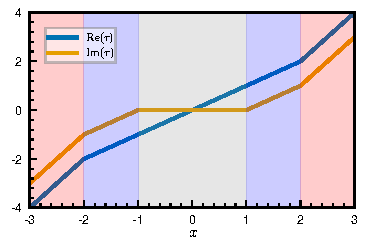
\includegraphics[width=0.5\textwidth]{figures/pml_real_and_imag.pdf}
  \caption{Real and imaginary part of change of variables corresponding
  to~\cref{eq:pml-with-stretching} with $\ell = L = 1$, $\sigma_0 = \sqrt{2}/2$,
  and $\mu_0 = 2$.}
  \label{fig:pml-with-stretching}
\end{figure}

While the form of the complex-stretching function can be commonly found in the
literature, the presence of the real-stretching is somewhat unusual; in the
context of the water-waves problem, it is related to the presence of evanescent
waves whose decay rate may be slower than  

To provide a heuristic for choosing $a,b,\mu_0$ and $\sigma_0$ given a desired
truncation tolerance $\epsilon$, we proceed as follows. First, the
complex-stretching strength $\sigma_0$ is chosen to be one; 

\subsection{Singular and nearly-singular integration} \label{sec:singular-integration}

\section{Numerical results}\label{sec:numerical-results}

In this section we present numerical results to illustrate the proposed method,
as well as to test the role of the various parameters. Unless otherwise state we
set $\omega^2/g =1$. All linear systems are solved by means of GMRES with a
relative tolerance of $10^{-12}$.

In our first example, we consider the semi-infinite domain $\R^+ \times [0,-h]$,
and impose a Neumann boundary condition on the $\Gamma_l = \{ 0 \} \times
[0,-h]$ curve corresponding to the Neumann trace of the modal solution
\begin{align}
  \phi(x_1,x_2) = \frac{\cosh(k(x_2+d))}{\cosh(kd)} e^{i k x_1} + \cos(\gamma_1(x_2+d)) e^{-\gamma_1 x_1},
\end{align}
where the first term represents a right-going (propagative) wave and the second
term is an evanescent mode. 

The depth $d$ is taken to be $1$, which yields $k \approx 1.2$ and
$\gamma_1=2.8$. 

From the
modal decomposition~\cref{eq:modaldecomp}, we know that
\begin{align}
  \varphi(x_1,x_2) = A_0^+u_0(x_2)e^{ik(x_1)} + \sum_{n\geq 1}A_n^+u_n(x_2)e^{-\gamma_n(x_1)},
\end{align}
is an exact solution of our problem. Taking its trace on $\Gamma_l$, we have our
problem setup.

\begin{figure}
  \centering
  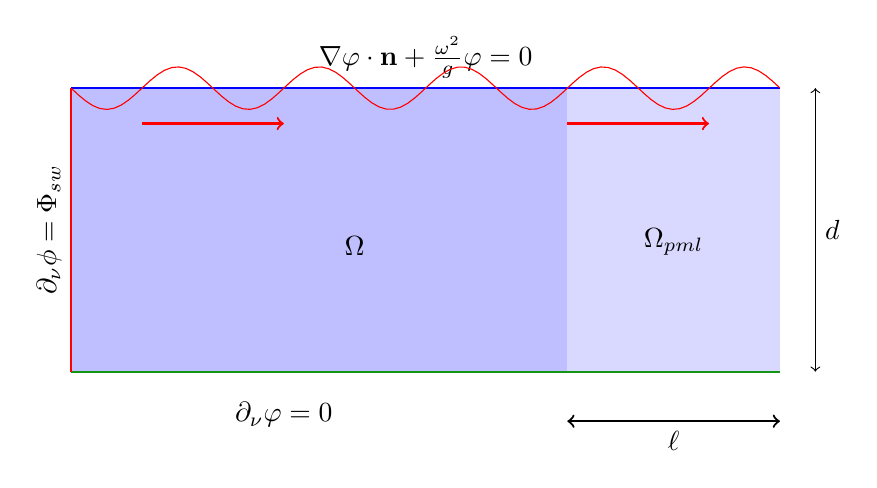
\begin{tikzpicture}[scale=0.9]
    \fill[color=blue!25] (-5,-4)--(5.,-4)--(5.,0)--(-5,0)--cycle;
    \fill[color=blue!15] (5,-4)-- (2,-4)--(2,0)
    --(5,0)--cycle;
    \draw[color=vertB,thick] (-5,-4)-- (5.,-4);
    \draw[color=red,thick] (-5,-4)-- (-5.,0);
  %	\fill[orange] (0,-2)ellipse(1. and 0.35);
  %	\fill[orange] (-.8,-2)--(-1.8,-2.5)--(-1.8 ,-1.5)--cycle;
    \draw[color=blue,thick] (5.,0)--(-5,0);
  %	\fill (.7,-2) ellipse(.05 and .05);
    \draw[above] (0,0) node{$\nabla \varphi \cdot \bn +
    \frac{\omega^2}{g}\varphi = 0$};
    \draw[above] (-1,-2.5) node{$\Omega$};
    \draw[above] (3.5,-2.5) node{$\Omega_{pml}$};
    \draw[below] (-2,-4.3) node{$\partial_{\nu}\varphi = 0$};	
    \draw[above] (-5,-2) node[rotate=90]{$\partial_{\nu} \phi = \Phi_{sw}$};
    \draw[<->] (5.5,-4)--(5.5,0);
    \draw[right] (5.5,-2) node{$d$};
    \draw[<->,thick] (5,-4.7) -- (2,-4.7);
    \draw[below] (3.5,-4.7) node{$\ell$};
    \draw[color=red, samples=100]  [domain=-5:5]  plot(\x, {.3*sin(3.14*\x r)});
    \draw[->,red,thick] (-4,-.5)--(-2,-.5);
    \draw[->,red,thick] (2,-.5)--(4,-.5);
  \end{tikzpicture}		  
  \caption{Schematic of wavemaker problem}
\end{figure}

In the first test we take $A_0 = 1$, $A_n = 0$ for $n\geq 1$, so that the
solution is simply the propagative mode. The results are show in figure ...

\begin{figure}
  \centering
  \begin{subfigure}{0.49\linewidth}
    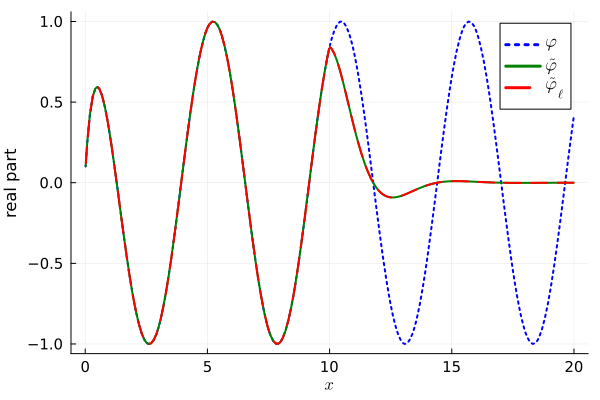
\includegraphics[width=1\textwidth]{figures/wavemaker_modal_solution.pdf}
    \caption{Behavior of the exact solution $\varphi$, its analytic extension
    $\tvarphi$, and the numerical (discrete) approximation $\tvarphi_{\ell,h}$.}
  \end{subfigure}
  \begin{subfigure}{0.49\linewidth}
    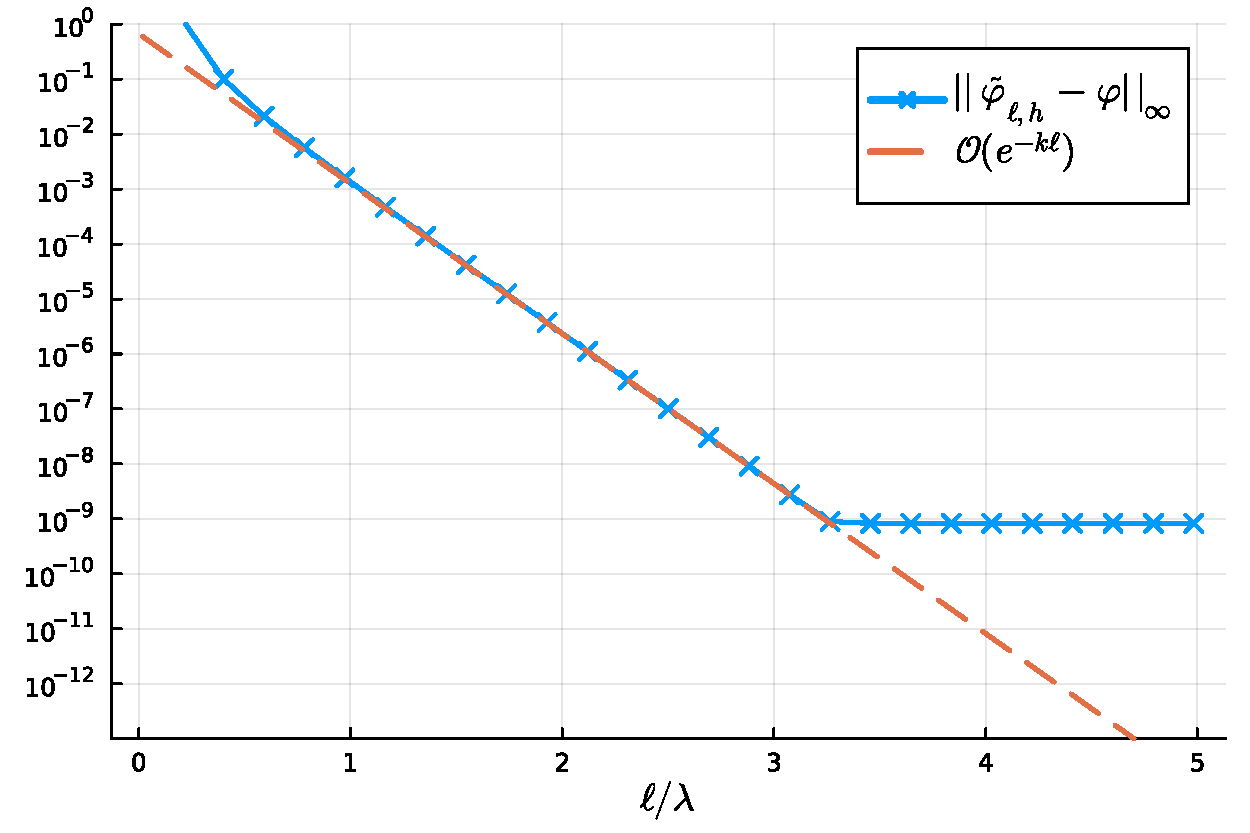
\includegraphics[width=1\textwidth]{figures/convergence_pml_planewave_depth_1.pdf}
    \caption{Convergence to exact solution as the length of the PML layer is increased.}
  \end{subfigure}
  \label{fig:convergence-sourcepoint}
  \caption{Convergence tests for a wavemaker with exact solution given by the sum of the propagative mode and the first evanescent mode for $h=1$ and $\omega^2/g = 1$. This gives $k \approx 1.2$ and $\gamma_1 \approx 2.8$. }
\end{figure}

As the depth is increased, we observe a change in the convergence behavior:

\begin{figure}
  \centering
  \begin{subfigure}{0.49\linewidth}
    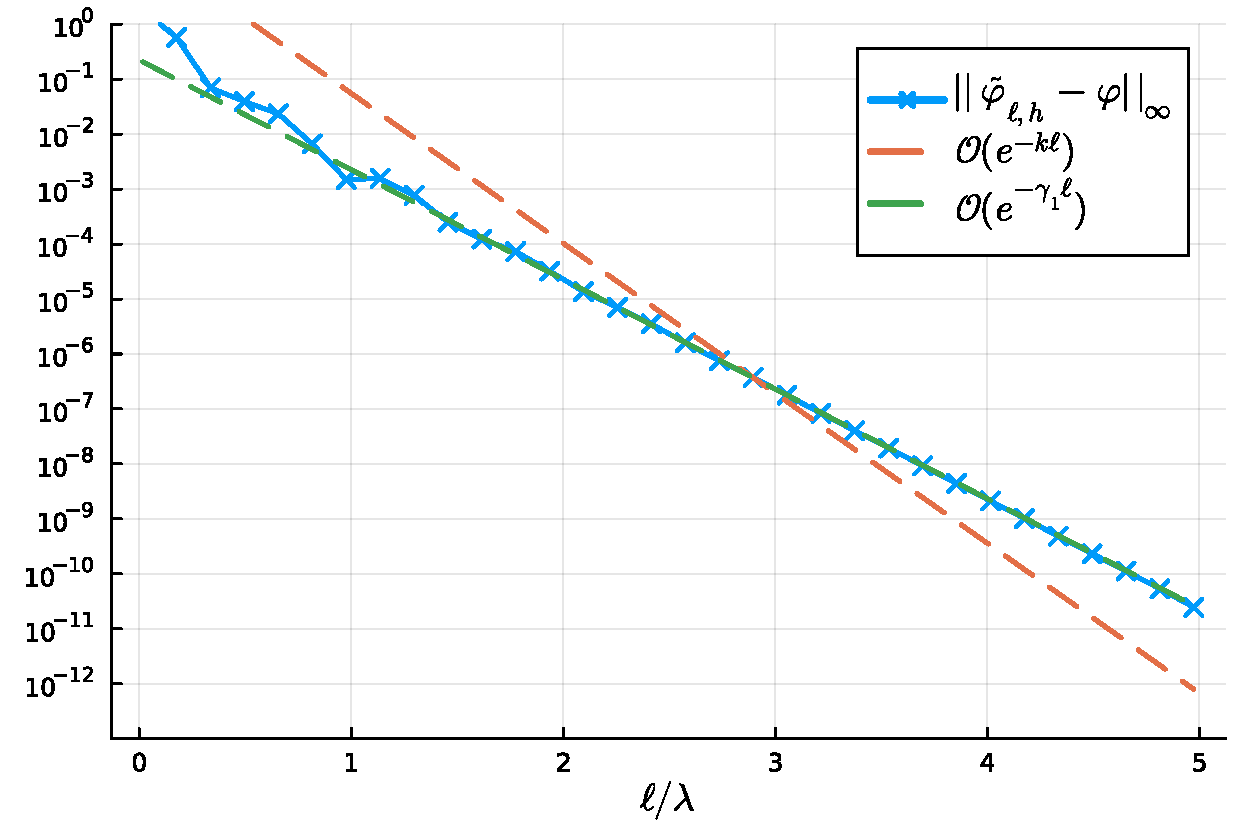
\includegraphics[width=\textwidth]{figures/convergence_pml_planewave_depth_3.pdf}
    \caption{Depth $d=3$, corresponding to $k \approx 1$, $\gamma_1 \approx 0.73$}
    \label{fig:convergence-modal-solution-depth-3}
  \end{subfigure}
  \begin{subfigure}{0.49\linewidth}
    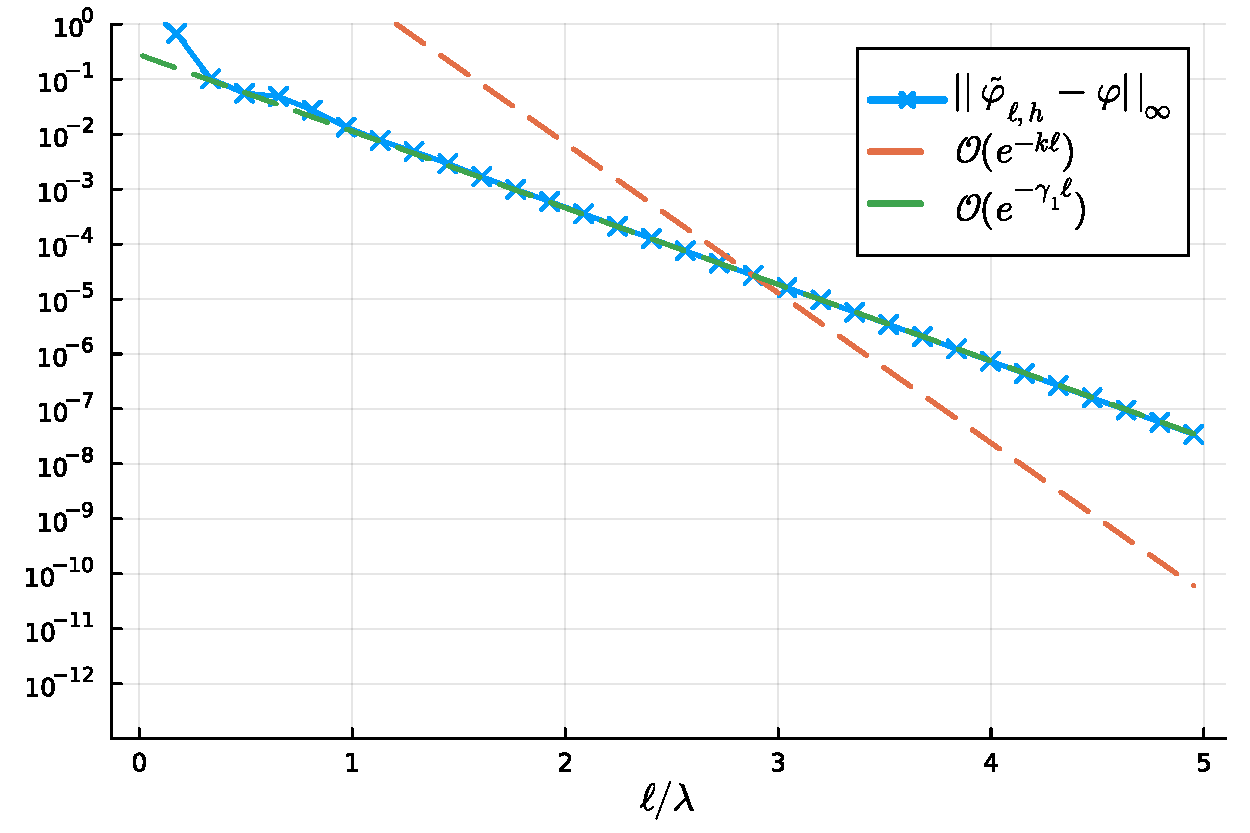
\includegraphics[width=1\textwidth]{figures/convergence_pml_planewave_depth_4.pdf}
    \caption{Depth $d=4$, corresponding to $k \approx 1$, $\gamma_1 \approx 0.51$}
    \label{fig:convergence-modal-solution-depth-4}
  \end{subfigure}
  \label{fig:convergence-modal-solution}
  \caption{Change in the convergence behavior as the depth $d$ is increased.}
\end{figure}

While not necessary, it is possible to further improve the convergence of the
method respect to the truncation parameter to obtain a $d$-independent result as
$d \to \infty$. To this end, it is necessary to modify $\tau$ so that it also
performs a real-stretching after the PML layer. 

With the real stretching, we can recover the expected convergence rate
of~\cref{fig:convergence-modal-solution-depth-4}
\begin{figure}
  \centering
  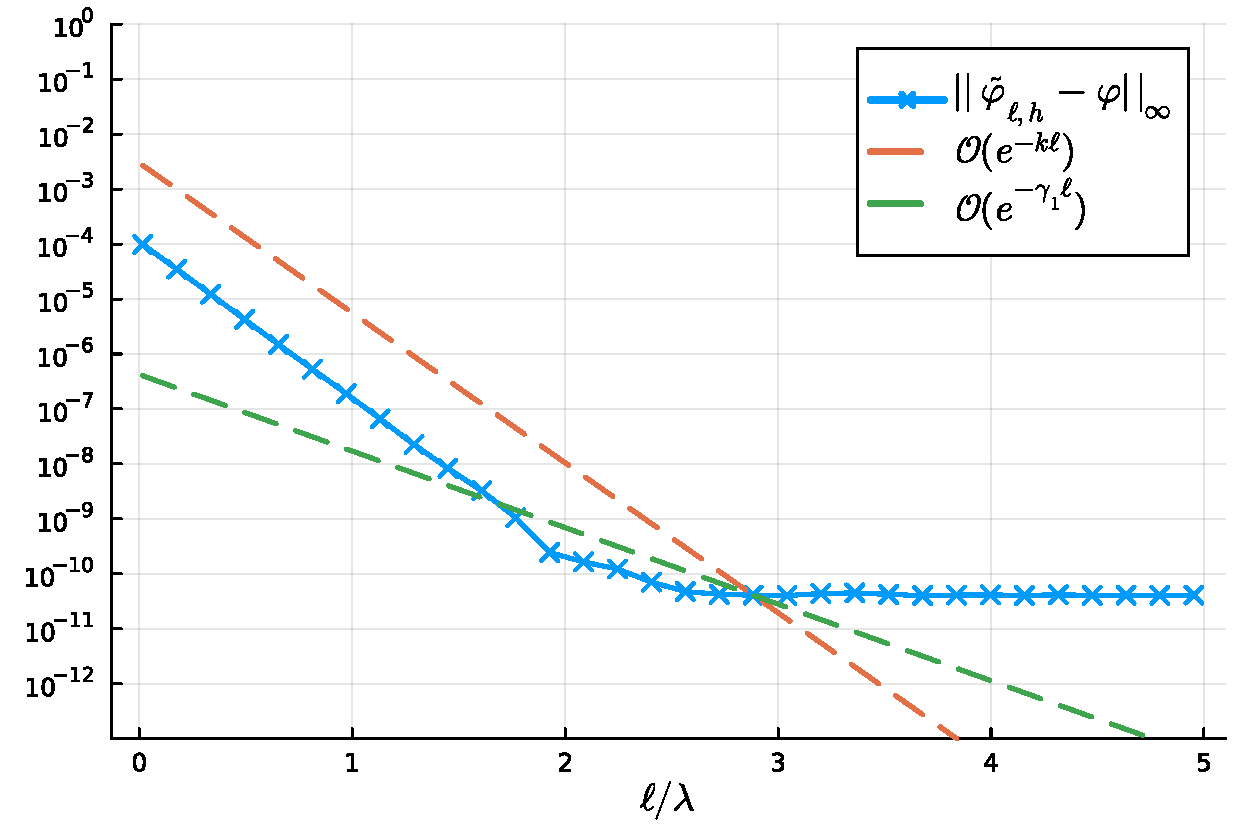
\includegraphics[width=0.5\textwidth]{figures/convergence_pml_stretching_planewave_depth_4.pdf}
  \caption{Convergence of modal solution with a stretching layer of length $\lambda$ and strength $d$ located after the PML to damp the evanescent mode. }
  \label{fig:pml-convergence-stretching-depth-4}
\end{figure}

\subsection{Mesh refinement}

Although not the main focus of this paper, we present in this subsection the
convergence results with respect to the mesh refinement. As mentioned
in~\cref{sec:singular-integration}, we use a composite quadrature rule to
discretize the surfaces, which in our code are represented by (explicit)
parametrisation. As mentioned, we use throughout this paper a $n$-point
Gauss-Legendre quadrature rule per element; such a quadrature rule exactly integrates
polynomials of order up to $2n-1$, yielding and the Gauss-Legendre nodes can be
used to interpolate a polynomial of order $n-1$. As mentioned
in~\cref{sec:singular-integration}, the expected convergence order is $()$


\begin{figure}
  \centering
  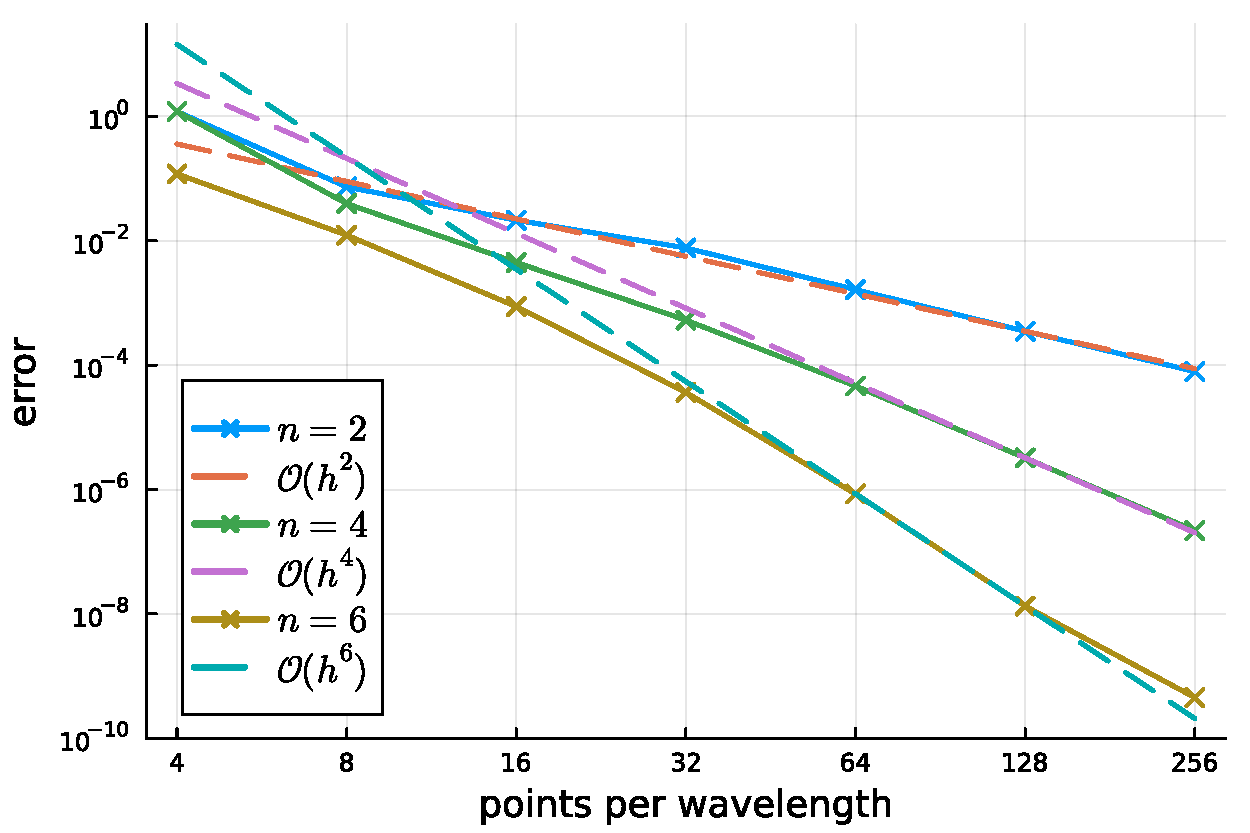
\includegraphics[width=0.5\textwidth]{figures/modal_convergence_meshsize_depth_1.pdf}
  \caption{Convergence to the modal solution as the number of points per wavelength is increased. The }
  \label{fig:mesh-convergence}
\end{figure}

\subsection{Scattering problem}



\appendix

\section{Ellipticity condition}\label{sec:elliptic-condition}

\begin{proposition}
  \label{pr:algebraic-condition-strongly-elliptic}
  The system \cref{eq:pml-laplace-real} is strongly elliptic if and only if
  $\mathrm{Re}(A)$ is positive definite.
\end{proposition}
\begin{proof}
  Since $A$ was assumed symmetric, it follows that
  \begin{align}
  2 \mathrm{Re}(\xi^* A \xi) = \xi^* A \xi + \overline{\xi^* A \xi}= \xi^* A \xi + \xi^* \bar{A} \xi = 2 \xi^* \mathrm{Re}(A) \xi
  \end{align}
  Splitting $\xi = \xi_r + i\xi_i$ into its real and imaginary parts, with
  $\xi_r,\xi_i \in \R^d$, we have that
  \begin{align}
  \xi^* \mathrm{Re}(A) \xi = \xi_r^t \mathrm{Re}(A) \xi_r + \xi_i^t \mathrm{Re}(A) \xi_i
  \end{align}
  If $\mathrm{Re}(A)$ is positive definite, we have that $\exists \delta > 0$ s.t.
  \begin{align}
  \xi^* \mathrm{Re}(A) \xi > \delta (\xi_r^2 + \xi_i^2) = \delta |\xi|^2
  \end{align}
  which proves the result one way. If $\mathrm{Re}(A)$ is not positive definite,
  then $\exists v \in \R^2$ s.t. $v^t \mathrm{Re}(A) v \leq 0$. Letting $\xi = v$
  the other direction is proved.
\end{proof}

\Cref{pr:algebraic-condition-strongly-elliptic} provides an algebraic criterion,
dependent only on the chosen change of variable $\btau$, to determine whether
\cref{eq:pml-laplace-real} is strongly elliptic on $\Omega$. 

\section{Complex-scaled fundamental solution}\label{sec:fundamental-solution}

We present a formal calculation to justify the fact that $\tilde{G}(\bx,\by) =G(\tau(\bx),\tau(\by))$ is the fundamental solution of
\begin{align}
  \nabla \cdot \left( \frac{1}{|J^{-1}|}J^{-1}(J^{-1})^t \nabla \tilde{G}(\bx,\by) \right) = \delta(\bx - \by),
  \quad \mbox{for} \quad \bx \in \R^2,
\end{align}

% We now investigate the asymptotic behavior of $\tilde{R}(\bx,\by) =
% R(\tau(\bx),\tau(\by))$ as $\by \to \bx$. First, we may write $\tau(\bx) -
% \tau(\by) = J(\bx)(\bx - \by) + \mathcal{O}(|\bx - \by|^2)$, so that
% \begin{align}
%   \tilde{R}^2(\bx,\by) &= (\tau(\bx) - \tau(\by)) \cdot (\tau(\bx) - \tau(\by)) + \mathcal{O}(R^4)\\
%               &= (\bx-\by)^t J(\bx)^t J(\bx) (\bx-\by) + \mathcal{O}(R^4)
% \end{align}
% This show in particular that, provided the eigenvalues of $J^tJ$ are s.t.
% $ 0< c < \lambda < C < \infty$, then $\tilde{R}$ goes to zero at the same rate
% as $R$.

% Finally, we will need the leading order term in the gradient of $\tilde{R}$. It
% is easier to use $\nabla(\tilde{R}\cdot\tilde{R}) = 2\tilde{R} \nabla\tilde{R}$
% so that we have
% \begin{align}
%   \nabla(\tilde{R}\cdot\tilde{R}) = \nabla((\bx - \by)^t J^t J (\bx - \by)) = 2 J^t J (\bx - \by) + \mathcal{O}(|\bx - \by|^2)
% \end{align}
% We are now ready to show the result.

% %
% First, take a test function $v \in \mathcal{D}(\Omega)$ and multiply and integrate:
% \begin{align}
%   \int_{\Omega} v(\bx) \left(\nabla \cdot \left( \frac{1}{|J^{-1}|}J^{-1}(J^{-1})^t \nabla \tilde{G}(\bx,\by) \right) + \frac{1}{|J^{-1}|}k^2\tilde{G}(\bx,\by)\right) \de \bx = v(\by)
% \end{align}
% Split the integral as $\int_\Omega = \int_{\Omega \setminus B_\epsilon(\bx)} + \int_{B_\epsilon(\bx)}$. Consider first the
% non-singular part:
% \begin{align}
%   I_1 = \int_{\Omega \setminus B_\epsilon(\bx)} v(\bx) \left(\nabla \cdot \left( \frac{1}{|J^{-1}|}J^{-1}(J^{-1})^t \nabla \tilde{G}(\bx,\by) \right) + \frac{1}{|J^{-1}|}k^2\tilde{G}(\bx,\by)\right) \de \bx
% \end{align}
% Noticing that the operator is in fact $|J|\tilde{\Delta}$, it follows by
% analyticity of $G$ (not clear to me) that $\tilde{\Delta} \tilde{G} + k^2
% \tilde{G} = 0$ for $\bx \neq \by$, and so $I_1 = 0$. Next we compute $I_2$.
% First note that the second term is has an integrable kernel, so it tends to zero as $\epsilon
% \to 0$. Applying the divergence theorem to the first term we obtain:
% \begin{align}
%   I_1 = -\int_{B_\epsilon(\by)} \nabla v(\bx) \cdot \left( \frac{1}{|J^{-1}|}J^{-1}(J^{-1})^t \nabla \tilde{G}(\bx,\by)\right) \de \bx  +
%   \int_{\partial B_{\epsilon}(\by)} v(\bx) A(\bx) \nabla \tilde{G}(\bx,\by) \cdot \bn \de s_\bx
% \end{align}
% The first part of $I_1$ is again integrable, so we need only estimate the second
% one. To compute the $\nabla \tilde{G}$ we use
% \begin{align}
%   \nabla \tilde{G}(\bx,\by) \sim \nabla \log (\tilde{R}(\bx,\by)) &= \frac{1}{\tilde{R}(\bx,\by)}\nabla \tilde{R}(\bx,\by) \\
%                                                                   &= \frac{1}{\tilde{R}^2(\bx,\by)}J^t(\bx)J(\bx)(\bx - \by)
% \end{align}
% Replacing this in the formula we get
% \begin{align}
%   I_1 =  \int_{\partial B_{\epsilon}(\by)} v(\bx) |J(\bx)| \frac{1}{(\bx-\by)^t J^t(\bx) J(\bx) (\bx - \by)} (\bx - \by)\cdot \bn \de s_\bx
% \end{align}
% Now parametrize the circle by $\bx = \by + \epsilon\br(\theta)$, with
% $\br(\theta) = (\cos(\theta),\sin(\theta))$, and replace $J(\bx) \approx
% J(\by)$, $\bn = \br$ to obtain
% \begin{align}
%   I_1 =  |J(\by)| v(\by)\int_0^{2\pi} \frac{1}{\br^t(\theta) J^t(\by) J(\by) \br(\theta)} \de \theta
% \end{align}
% The last thing is thus to compute the integral
% \begin{align}
%   \int_0^{2\pi} \frac{1}{\br^t(\theta) J^t(\by) J(\by) \br(\theta)} \de \theta.
% \end{align}

% Letting $J = [a b; c d]$, we can compute


% For the two-dimensional problem, we have that 
% \begin{align}
%   J = \begin{bmatrix}
%     \tau_{1,1} & \tau_{1,2}\\
%     0 & 1
%   \end{bmatrix}
%   ,\quad 
%   J^{-1} = \begin{bmatrix}
%     1/\tau_{1,1} & -\tau_{1,2}/\tau_{1,1}\\
%     0 & 1
%   \end{bmatrix}
% \end{align}
% and so
% \begin{align}
%   A = |J|J^{-1}(J^{-1})^t = 
%   \frac{1}{\tau_{1,1}}
%   \begin{bmatrix}
%     1 + \tau_{1,2}^2 & -\tau_{1,2}\tau_{1,1} \\
%     -\tau_{1,2}\tau_{1,1} & \tau_{1,1}^2
%   \end{bmatrix}
% \end{align}
% Assuming $\tau_{1,2}$ is purely imaginary, we have that
% \begin{align}
%   \mathrm{Re}(A) = 
%   \begin{bmatrix}
%     \mathrm{Re}\left(\frac{1 + \tau_{1,2}^2}{\tau_{1,1}}\right) & 0 \\
%     0 & \mathrm{Re}(\tau_{1,1})
%   \end{bmatrix}
% \end{align}
% Considering a change of variables of the form $\tau_i = x_i + i\sigma_i(\bx)$,
% we arrive at the following simple condition:
% \begin{align}
%   |\sigma_{1,2}| < 1
% \end{align}


% While in \cref{sec:orthogonal-pml} we considered the special case where
% $\tau(\bx) = (\tau_1(x_1),\tau_2(x_2))$, we present now the generic case with
% $\tau(\bx) = (\tau_1(\bx),\tau_2(\bx))$. The matrix $A$ is then given by
% \begin{align}
%   A = \frac{1}{|J|}
%   \begin{bmatrix}
%     \tau_{2,2}^2 + \tau_{1,2}^2 & -\tau_{2,1}\tau_{2,2} - \tau_{1,2}\tau_{1,1} \\
%     -\tau_{2,1}\tau_{2,2} - \tau_{1,2}\tau_{1,1}  & \tau_{1,1}^2 + \tau_{2,1}^2
%   \end{bmatrix},
% \end{align}

% Determining ellipticity of this matrix (i.e. finding conditions on $\tau$ under
% which $\mathrm{Re}(A)$ is positive definite) in the general case is a somewhat
% cumbersome calculation which we deferred to \cref{sec:ellipticity-of-A}. For the
% numerical examples we consider in \cref{sec:numerical-examples}, it suffices to
% focus on the uni-axial (but non-orthogonal) case, where we assume $\tau_2(\bx) =
% x_2$. The matrix $A$ then simplifies to
% \begin{align}
%   A  =   \begin{bmatrix}
%     \frac{1 - \sigma_{1,2}^2}{1 + i\sigma_{1,1}} & -i\sigma_{1,2} \\
%     -i\sigma_{1,2} & 1 + i\sigma_{1,1}
%   \end{bmatrix}, \quad
%                      \mathrm{Re}(A) =   \begin{bmatrix}
%     \frac{1 - \sigma_{1,2}^2}{1+\sigma_{1,1}^2} & 0 \\
%     0 & 1
%   \end{bmatrix},
% \end{align}
% %
% and strong ellipticity is equivalent to the simple condition:
% \begin{align}
%   \label{eq:ellipticity-condition-nonorthogonal}
%   \left| \sigma_{1,2}(\bx) \right| < 1 \quad \mbox{for all} \quad \bx \in \Omega.
% \end{align}

% In order to give a geometric interpretation to this condition, it is useful to
% consider a simple case given by
% \begin{align}
%   \tau_1 =
%   \begin{cases}
%     x_1 + i \beta (x_1 + \frac{1}{\alpha} x_2 + a) \quad &\mbox{for} \quad x_1 < -\frac{1}{\alpha} x_2 - a, \\
%     x_1 \quad &\mbox{for} \quad |x_1| < \frac{1}{\alpha} x_2 + a, \\
%     x_1 + i \beta (x_1 - \frac{1}{\alpha} x_2 - a) \quad &\mbox{for} \quad x_1 > \frac{1}{\alpha} x_2 + a.
%   \end{cases}
% \end{align}
% The parameters $\alpha$ and $a$ determine the region where the PML is applied,
% and the parameter $\beta$ controls the attenuation strength inside the PML layer
% (see \cref{fig:sch-pml}). By taking taking the limit $\alpha \to \infty$, for
% instance, we recover the case of an orthogonal PML discussed in
% \cref{sec:orthogonal-pml}.

% We are interested in the analytic extension of $\varphi$ when it is
% exponentially decaying at infinity. This leads to consider the analytic
% extension of $\varphi$ for $\Re(x_1)>L$  (resp. $\Re(x_1)<-L$) only for
% $\Im(x_1)>0$ (resp. $\Im(x_1)<0$), so that the propagating surface mode becomes
% exponentially decaying at infinity. Letting $\btau : \R^2 \to
% \C^2$ mapping points $\bx$ on the physical domain to $\tilde{\bx} = \btau(\bx)$.
% Then, assuming that $\tau(\bx)$ is the identity map for $|x_1|<L$, and defining
% $\tilde{\varphi}(x_1,x_2) = \varphi(\tau(x_1),x_2)$ as the analytic 

\bibliographystyle{abbrv}
\bibliography{references}

\end{document}
